\documentclass[fleqn]{article}

\usepackage{listings}
\usepackage{diagbox}
\usepackage[german]{babel}
\usepackage[T1]{fontenc}
\usepackage[latin1]{inputenc}
\usepackage{titlesec}
\usepackage{geometry}
\usepackage{qtree}
\usepackage{tikz}
\usepackage{amsmath}
\usepackage{amssymb}
\setcounter{secnumdepth}{0}
\usetikzlibrary{positioning}
\geometry{top=2.5cm, bottom=2.5cm}
\lstset{
 columns=fixed,       
 numbers=left,                                        % 在左侧显示行号
 numberstyle=\tiny\color{gray},                       % 设定行号格式
 frame=none,                                          % 不显示背景边框
 backgroundcolor=\color[RGB]{245,245,244},            % 设定背景颜色
 keywordstyle=\color[RGB]{40,40,255},                 % 设定关键字颜色
 numberstyle=\footnotesize\color{darkgray},           
 commentstyle=\it\color[RGB]{0,96,96},                % 设置代码注释的格式
 stringstyle=\rmfamily\slshape\color[RGB]{128,0,0},   % 设置字符串格式
 showstringspaces=false,                              % 不显示字符串中的空格
 language=c++,                                        % 设置语言
 breaklines,                                          % 自动换行
}

\title{TU Chemnitz \\ Praktikum Grundlagen Technische Informatik \\ Versuch Sequ2}

\author{Gruppe 5 - Team 5: \\ Dongze Yang \\Xiangyu Tong \\ Treshchun Kateryna}

\begin{document}

\maketitle



\newpagestyle{main}{
    \sethead{}{}{Grupe 5 - Team 5}
    \setfoot{}{\thepage}{}
    \headrule
    \footrule
}
\pagestyle{main}
%\section{Aufgabe}

\section{Statische Funktionen}

-Rücksetzen in den Zustand 11

\noindent-Laden 2-Bit-Zahl

\subsection{Rücksetzen in den Zustand 11}

\begin{center}
    \begin{tabular}{c|c|c|c|c}
        Re&Q&Q'&S&R\\
        \hline
        0&0&0&0&-\\
        0&1&1&-&0\\
        1&0&1&1&0\\
        1&1&1&-&0
    \end{tabular}
    $\qquad \Rightarrow\qquad S=Re,R=0$
\end{center}

\subsection{Laden 2-Bit-Zahl}

\begin{center}
    \begin{tabular}{c|c|c|c|c|c}
        LO&D&Q&Q'&S&R\\
        \hline
        0&0&0&0&0&-\\
        0&0&1&1&-&0\\
        0&1&0&0&0&-\\
        0&1&1&1&-&0\\
        1&0&0&0&0&-\\
        1&0&1&0&0&1\\
        1&1&0&1&1&0\\
        1&1&1&1&-&0
    \end{tabular}
    $\qquad\Rightarrow\qquad S=LO\cdot D,R=\overline{D}\cdot LO $
    
    $R= R + \overline{LO}\cdot LO = (\overline{D}+\overline{LO})\cdot LO = \overline{D\cdot LO}\cdot LO = \overline{S}\cdot LO$
    
\end{center}

\subsection{Superposition}

$S_i = D_i\cdot LO + Re \Rightarrow \overline{S_i} = \overline{\overline{\overline{D_i\cdot LO}\cdot \overline{Re}}}$

\noindent$R_i = \overline{S_i}\cdot LO + 0 \Rightarrow \overline{R_i} = \overline{\overline{S}\cdot LO}$

\section{Dynamische Funktionen}

-Rückwärtszählen

\noindent-Linksschieben

\subsection{Rückwärtszählen}

\begin{center}
    \begin{tabular}{cc|cc|cc|cc}
        Q1&Q0&Q1'&Q0'&J1&K1&J0&K0\\
        \hline
        0&0&1&1&1&-&1&-\\
        0&1&0&0&0&-&-&1\\
        1&0&0&1&-&1&1&-\\
        1&1&1&0&-&0&-&1\\
    \end{tabular}
    $\qquad \Rightarrow \qquad J0=1,K0=1,J1=\overline{Q0},K1=\overline{Q0}$
\end{center}

\subsection{Linksschieben}

\begin{center}
    \begin{tabular}{cc|cc|cc|cc}
        Q1&Q0&Q1'&Q0'&J1&K1&J0&K0\\
        \hline
        0&0&0&1&0&-&1&-\\
        0&1&1&1&1&-&-&0\\
        1&0&0&1&-&1&1&-\\
        1&1&1&1&-&0&-&0
    \end{tabular}
    $\qquad\Rightarrow\qquad J0=1,K0=0,J1=Q0,K1=\overline{Q0}$
\end{center}

\subsection{Superposition}

\begin{center}
    \begin{tabular}{c|cc|cc|cc}
        Funktion&CB&SL&J1&K1&J0&K0\\
        \hline
        keine Funktion aktiviert&0&0&0&0&0&0\\
        \hline
        Rückwärtszählen(CB)&1&0&$\overline{Q0}$&$\overline{Q0}$&1&1\\
        \hline
        Linksschieben(SL)&0&1&$Q0$&$\overline{Q0}$&1&0
    \end{tabular}
\end{center}

$J1=\overline{CB}\cdot\overline{SL}\cdot 0 + CB\cdot\overline{SL}\cdot\overline{Q0} + \overline{CB}\cdot SL\cdot Q0$

$K1=\overline{CB}\cdot\overline{SL}\cdot 0 + CB\cdot\overline{SL}\cdot\overline{Q0} + \overline{CB}\cdot SL\cdot \overline{Q0}$

$J0=\overline{CB}\cdot\overline{SL}\cdot 0 + CB\cdot\overline{SL}\cdot1 + \overline{CB}\cdot SL\cdot 1$

$K0=\overline{CB}\cdot\overline{SL}\cdot 0 + CB\cdot\overline{SL}\cdot1 + \overline{CB}\cdot SL\cdot 0$

\qquad $\Downarrow$

$J1=CB\cdot\overline{Q0}+SL\cdot Q0 = \overline{\overline{CB\cdot\overline{Q0}}\cdot\overline{SL\cdot Q0}}$

$K1=CB\cdot\overline{Q0}+SL\cdot\overline{Q0} = \overline{\overline{CB\cdot \overline{Q0}}\cdot\overline{SL\cdot\overline{Q0}}}$

$J0=CB+SL = \overline{\overline{CB}\cdot\overline{SL}}$

$K0=CB$

\section{Schaltplan}

\begin{center}
        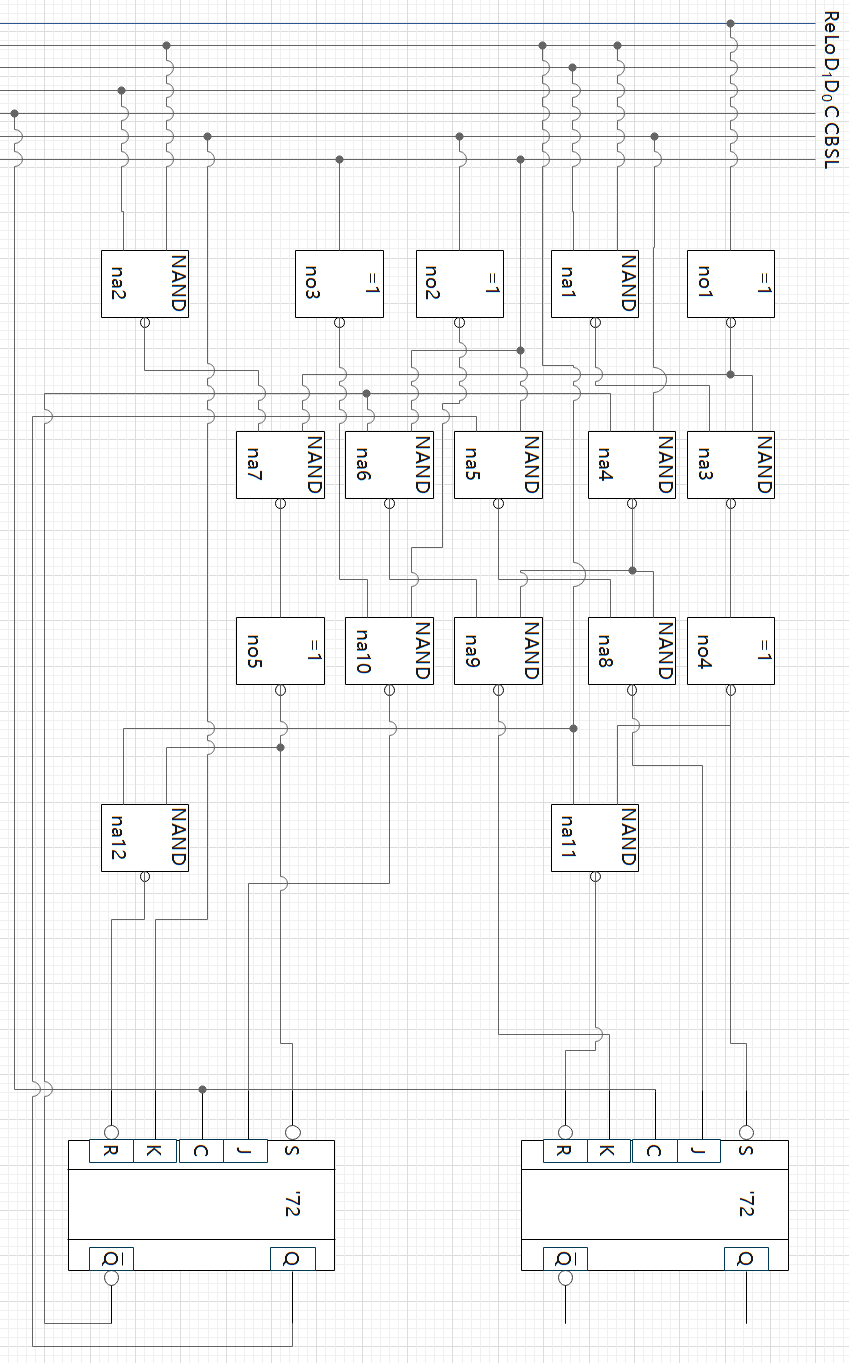
\includegraphics[scale=0.6]{bild1.png}
\end{center}

\section{VHDL-Strukturbeschreibung}

\begin{lstlisting}
library ieee;
use ieee.std_logic_1164.all;                               
use work.pack_2.all;                                       
                                                            
entity uut is                                            
    port (EE_X : in  X01_vector(7 downto 0);
        EE_Y : out X01_vector(23 downto 16));       
end uut;     

architecture structure of uut is
    component sn7400 -- 2er-nand 
        port (x : in X01_vector (1 to 2); 
            y : out X01); 
    end component; 

    component sn7404 is -- not 
        port (x : in X01; 
            y : out X01); 
    end component; 

    component sn7472 is -- JK-MS-Flipflop 
        port (s_b,r_b,c : in X01; 
            j,k : in X01_vector(1 to 3); 
            q,q_b : out X01); 
    end component;

    alias c     : X01 is EE_X(0);
    alias sl    : X01 is EE_X(1);
    alias cb    : X01 is EE_X(2);
    alias reset : X01 is EE_X(4);

    alias load  : X01 is EE_X(5);
    alias d1    : X01 is EE_X(6);
    alias d0    : X01 is EE_X(7);

    alias q1    : X01 is EE_Y(17);
    alias q0    : X01 is EE_Y(16);

    signal n1,n2,n3,n4,n5,n6 : X01; 

    signal nand1,nand2,nand3,nand4,nand5,nand6,nand7,nand8,nand9,nand10,nand11,nand12 : X01;

    signal fq0,nq0 : X01;

begin
    

    no1: sn7404 port map(x=>reset,y=>n1);
    no2: sn7404 port map(x=>cb,y=>n2);
    no3: sn7404 port map(x=>sl,y=>n3);
    no4: sn7404 port map(x=>nand3,y=>n4);
    no5: sn7404 port map(x=>nand7,y=>n5);
    
    na1: sn7400 port map(x(1)=>load,x(2)=>d1,y=>nand1);
    na2: sn7400 port map(x(1)=>load,x(2)=>d0,y=>nand2);
    na3: sn7400 port map(x(1)=>n1,x(2)=>nand1,y=>nand3);
    na4: sn7400 port map(x(1)=>cb,x(2)=>nq0,y=>nand4);
    na5: sn7400 port map(x(1)=>sl,x(2)=>fq0,y=>nand5);
    na6: sn7400 port map(x(1)=>sl,x(2)=>nq0,y=>nand6);
    na7: sn7400 port map(x(1)=>n1,x(2)=>nand2,y=>nand7);
    na8: sn7400 port map(x(1)=>nand4,x(2)=>nand5,y=>nand8);
    na9: sn7400 port map(x(1)=>nand4,x(2)=>nand6,y=>nand9);
    na10: sn7400 port map(x(1)=>n2,x(2)=>n3,y=>nand10);
    na11: sn7400 port map(x(1)=>n4,x(2)=>load,y=>nand11);
    na12: sn7400 port map(x(1)=>n5,x(2)=>load,y=>nand12);
    
    
    
    --ffq1:
    ff1: sn7472 port map(s_b=>n4,r_b=>nand11,c=>c,j(1)=>nand8,j(2)=>'1',j(3)=>'1',k(1)=>nand9,k(2)=>'1',k(3)=>'1',q=>q1);

    --ffq0:
    ff2: sn7472 port map(s_b=>n5,r_b=>nand12,c=>c,j(1)=>nand10,j(2)=>'1',j(3)=>'1',k(1)=>cb,k(2)=>'1',k(3)=>'1',q=>fq0,q_b=>nq0);
    q0 <= fq0;
end structure;
\end{lstlisting}

\section{Stimulation}

\subsection{Binäre Stimulationsfolge}
C SL CB Reset - Load D1 D0
\begin{lstlisting}
stimmap dbb2_08 000-0000|xx------
stimmap dbb2_08 000-1000|11------
stimmap dbb2_08 000-0000|11------
stimmap dbb2_08 001-0000|11------
stimmap dbb2_08 101-0000|11------
stimmap dbb2_08 001-0000|10------
stimmap dbb2_08 101-0000|10------
stimmap dbb2_08 001-0000|01------
stimmap dbb2_08 101-0000|01------
stimmap dbb2_08 001-0000|00------
stimmap dbb2_08 101-0000|00------
stimmap dbb2_08 001-0000|11------
stimmap dbb2_08 101-0000|11------
stimmap dbb2_08 000-0000|11------
stimmap dbb2_08 000-0100|00------
stimmap dbb2_08 100-0100|00------
stimmap dbb2_08 000-0101|01------
stimmap dbb2_08 100-0101|01------
stimmap dbb2_08 000-0111|11------
stimmap dbb2_08 100-0111|11------
stimmap dbb2_08 000-0110|10------
stimmap dbb2_08 100-0110|10------
stimmap dbb2_08 000-0000|10------
stimmap dbb2_08 010-0000|10------
stimmap dbb2_08 110-0000|10------
stimmap dbb2_08 010-0000|01------
stimmap dbb2_08 110-0000|01------
stimmap dbb2_08 010-0000|11------
stimmap dbb2_08 110-0000|11------
\end{lstlisting}

\subsection{Ternäre Stimulationsfolge}

\begin{lstlisting}
stimmap dbb2_08 000−0000|xx−−−−−
stimmap dbb2_08 000−1000|11−−−−−
stimmap dbb2_08 000−x000|--−−−−−
stimmap dbb2_08 000−0000|11−−−−−
stimmap dbb2_08 00x−0000|--−−−−−
stimmap dbb2_08 001−0000|11−−−−−
stimmap dbb2_08 101−0000|11−−−−−
stimmap dbb2_08 001−0000|10−−−−−
stimmap dbb2_08 101−0000|10−−−−−
stimmap dbb2_08 001−0000|01−−−−−
stimmap dbb2_08 101−0000|01−−−−−
stimmap dbb2_08 001−0000|00−−−−−
stimmap dbb2_08 101−0000|00−−−−−
stimmap dbb2_08 001−0000|11−−−−−
stimmap dbb2_08 101−0000|11−−−−−
stimmap dbb2_08 x0x−0000|--−−−−−
stimmap dbb2_08 000−0000|11−−−−−
stimmap dbb2_08 000−0x00|--−−−−−
stimmap dbb2_08 000−0100|00−−−−−
stimmap dbb2_08 100−0100|00−−−−−
stimmap dbb2_08 000−0101|01−−−−−
stimmap dbb2_08 100−0101|01−−−−−
stimmap dbb2_08 000−0111|11−−−−−
stimmap dbb2_08 100−0111|11−−−−−
stimmap dbb2_08 000−0110|10−−−−−
stimmap dbb2_08 100−0110|10−−−−−
stimmap dbb2_08 x00−0xx0|--−−−−−
stimmap dbb2_08 000−0000|10−−−−−
stimmap dbb2_08 0x0−0000|--−−−−−
stimmap dbb2_08 010−0000|10−−−−−
stimmap dbb2_08 110−0000|10−−−−−
stimmap dbb2_08 010−0000|01−−−−−
stimmap dbb2_08 110−0000|01−−−−−
stimmap dbb2_08 010−0000|11−−−−−
stimmap dbb2_08 110−0000|11−−−−−    
\end{lstlisting}

\end{document}